\subsection{Distance Estimation Pipeline}

This project applies a metric distance estimation pipeline, developed by Haucke et al.\cite{HAUCKE2022101536},
to the endeavour of monocular depth estimation (MDE) of chimpanzee-to-camera distances in images
sampled from camera trap video in the WCF dataset.
Four distinct parameterisations of this pipeline are used (Figure~\ref{fig:distance_pipeline}) to
generate four sets of distance data, combining either Dense Prediction Transformers\cite{dpt} (DPT)
or Depth Anything \cite{depth_anything} models for MDE with either Mega Detector\cite{mega_detector}
or both Mega Detector and Segment Anything\cite{segment_anything} used for collectively detection and
pixel sampling.

\vspace{5mm}

\begin{figure}[H]
    \centering
    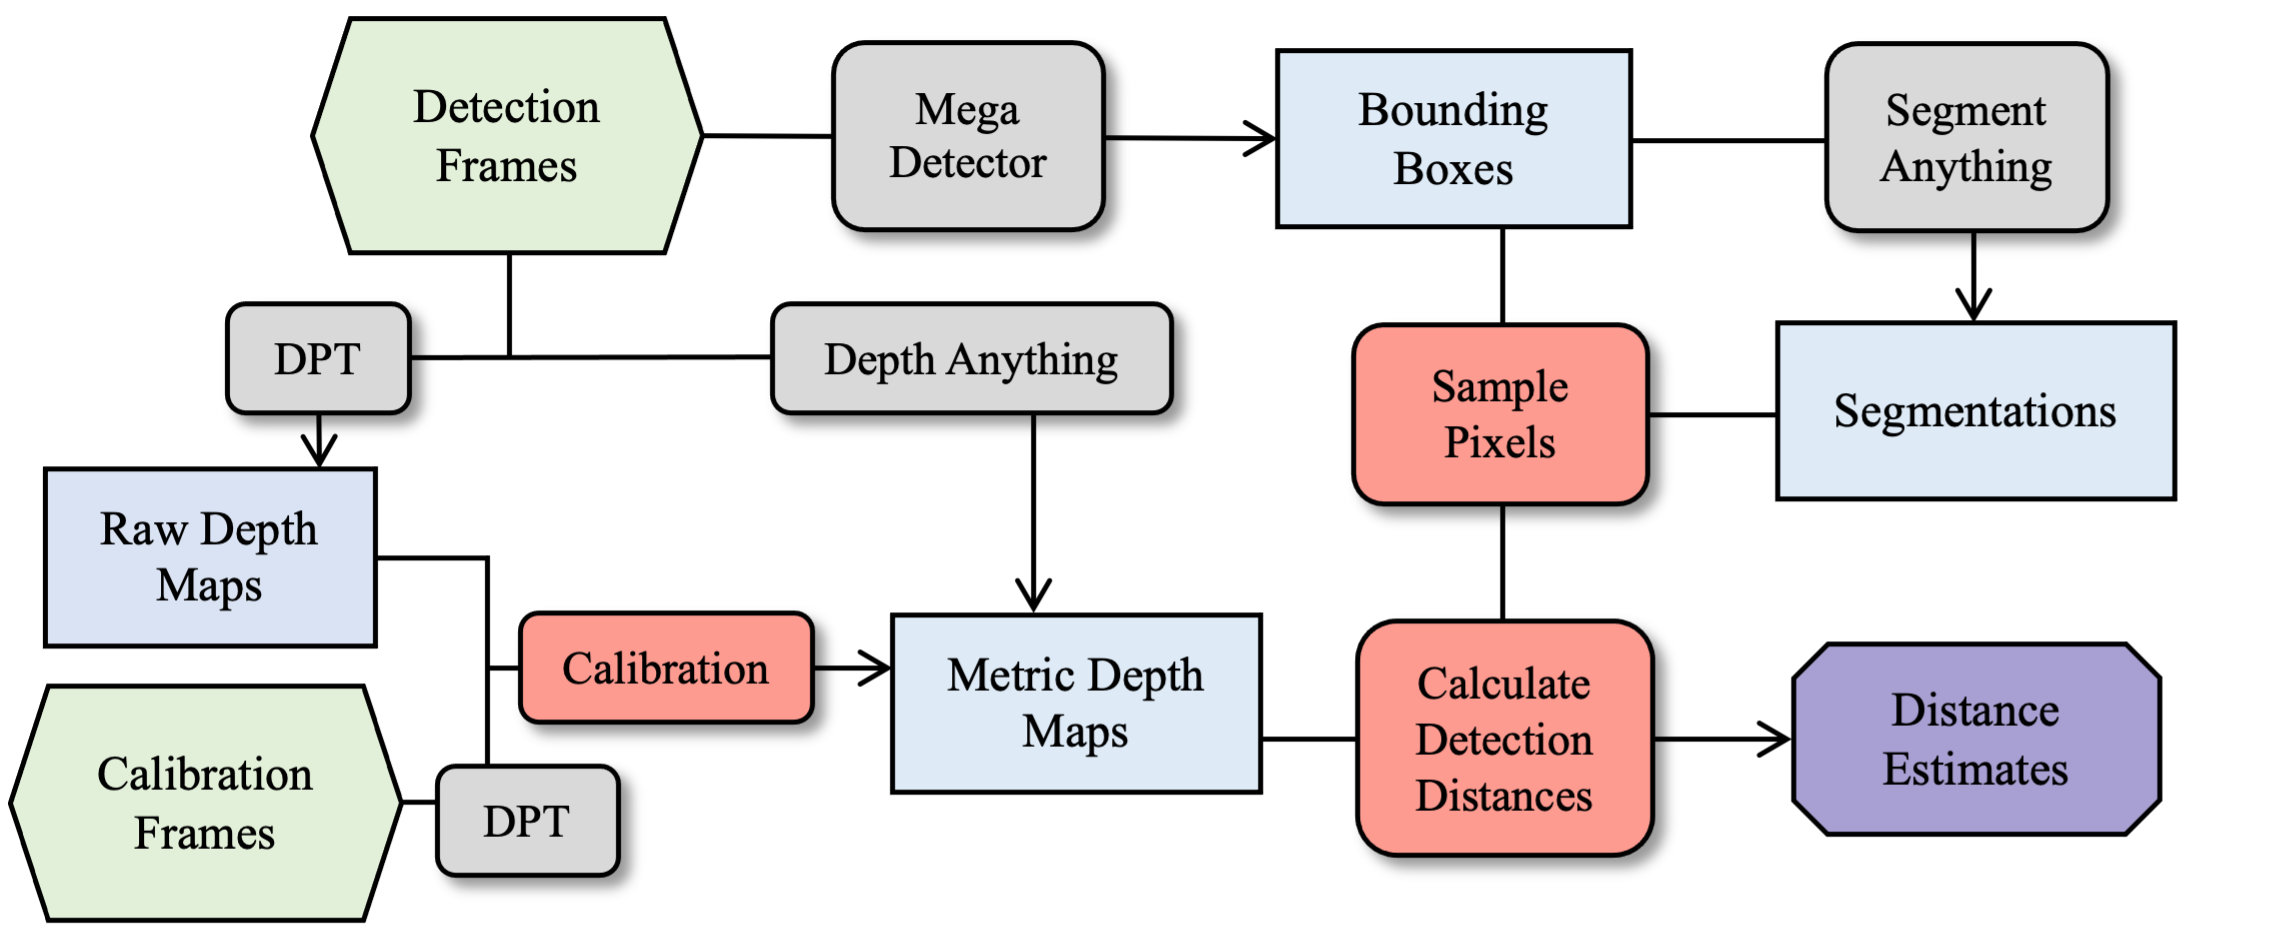
\includegraphics[width=0.9\textwidth]{body/background/assets/distance_pipeline}
    \vspace{3mm}
    \caption{Flowchart illustrating the overall workflow of the distance estimation pipeline.
    The MDE model generates depth maps corresponding to the detection frames. In the case of
    DPT, the outputted depth maps are each calibrated by aligning the depth scale to the
    average depth of the calibration frames to give corresponding metric depth maps.
    Mega detector then identifies bounding boxes within the detection frames with Segment
    Anything then optionally generating detection segmentations within these bounding boxes.
    The depth estimates of the pixels defined by the bounding boxes/segmentations given by
    the corresponding depth maps used finally used to calculate depth estimates.}
    \label{fig:distance_pipeline}
\end{figure}

\subsubsection{Dense Prediction Transformers}\label{subsubsec:dpt}

\textbf{DPT vs Conventional Architecture}

DPT, introduced by Ranftl et al.\cite{dpt}, is a (novel at conception) deep learning architecture
for dense prediction tasks, adapting the conventional convolutional encoder/decoder architecture
typically used for dense prediction\cite{segmentation_CNN,invariant_CNNs}
(i.e., the labelling of all pixels in an image), by substituting the encoder with a series of staged
vision transformers\cite{vision_transformer,transformer}.
This proves to be beneficial for tasks involving dense prediction (i.e., MDE) as the network retains
global context of the image and high feature resolution through all transformer stages\cite{dpt,transformer}.
This is not the case with convolutional neural networks, where features at progressively higher levels of
abstraction in the image are captured through repeated down-sampling over convolutional layers, resulting
in a loss of detail at deeper layers where the context is larger\cite{dpt,invariance_in_CNNs}.

\clearpage
\textbf{Training}

The vision transformer backbone of the network is pretrained with weights obtained using the ImageNet
dataset while the convolutional decoder weights are randomised\cite{dpt,imagenet}.
For the application to MDE in this pipeline, the model is trained on an extremely large aggregate
dataset of approximately 1.4 million images, leveraging a technique referred to as 'zero-shot
cross dataset transfer'.
This technique employs loss functions that are compatible with training data obtained using a range
ground-truth assessment methods (e.g., stereo cameras, lasers, structured-light 3D scanners) with
differing scales and shits.
As a consequence, raw DPT output should be considered as a measure of relative distance\cite{dpt,dpt_training}.

\vspace{5mm}
\textbf{Metric Calibration}

To achieve metric distance estimates from DPT, enabling application in distance sampling,
the model is fine-tuned to account for differences in depth scale and shift at each individual
camera location.
This is done by calibrating to location-specific ground-truth data.
For each camera location, a set of calibration frames and corresponding binary segmentation masks
are required (Figure~\ref{fig:dpt_cal_frames}).
Each calibration frame depicts a person/object (referred to as a 'landmark') positioned at a
known distance from the camera.
Each binary mask corresponds to a single calibration frame and depicts a segmentation of the
corresponding landmark, where all pixels inside the segmentation are coloured white with all
remaining pixels being coloured black.\cite{HAUCKE2022101536}

\vspace{5mm}

\begin{figure}[H]
    \centering
    \begin{subfigure}[t]{0.48\textwidth}
        \centering
        \includegraphics[height=0.16\textheight]{body/background/assets/calibration/raw}
    \end{subfigure}
    \begin{subfigure}[t]{0.48\textwidth}
        \centering
        \includegraphics[height=0.16\textheight]{body/background/assets/calibration/mask}
    \end{subfigure}

    \caption{Example a DPT calibration frame (left) and corresponding binary mask (right) at 2 meters.
        the binary mask shows a pixel-wise segmentation of the frame landmark, where occluding tree
        branch is excluded from the segmentation.}
    \label{fig:dpt_cal_frames}
\end{figure}

The following calibration method is a summary of the techniques described by
Haucke et al.\cite{HAUCKE2022101536}:

The $N$ total calibration frames are first run through DPT to generate raw disparity maps corresponding to
each frame.
The scale, $m_i$, and shift, $c_i$, of the calibration function (of form $y = mx + c$) mapping the raw
disparity output to calibrated disparity (equal to inverse metric distance) for the $N^\mathrm{th}$ frame
are calculated such that
\[
    (m_i,c_i) \approx \argmin_{m_i,c_i} \sum_{i=1}^{N-1} |m_i \cdot \textbf{D}_i^{ref}(\textbf{M}_i^{ref}=0) + c_i - \textbf{D}_N^{ref}(\textbf{M}_N^{ref}=0)|
\]
where $\textbf{D}_i^{ref}(\textbf{M}_i^{ref}=0)$ is all pixels in the disparity map $\textbf{D}_i^{ref}$
outside the binary mask $\textbf{M}_i^{ref}$.
With these computed scales and shifts for each calibration frame, the overall scale, $m$, and shift, $c$,
for the calibration function mapping the raw disparity output to calibrated disparity for the whole camera
location are calculated such that
\[
    (m,c) \approx \argmin_{m,c} \sum_{i=1}^{N} |m \cdot \mathrm{median}(m_i \cdot \textbf{D}_i^{ref}(\textbf{M}_i^{ref}=1) + c_i ) + c - \dfrac{1}{z_i}|
\]
where $\textbf{D}_i^{ref}(\textbf{M}_i^{ref}=1)$ is all pixels in the disparity map $\textbf{D}_i^{ref}$
enclosed within the binary mask $\textbf{M}_i^{ref}$ and $z_i$ is the ground-truth distance.
The shift and scale values of the disparity map $\textbf{D}_N^{ref}$ are, by definition, $m_N = 1$ and $c_N = 0$.

The final calibrated disparity maps, $\textbf{C}_i^{ref}$, and metric depth maps, $\textbf{Z}_N^{ref}$,
for the camera location reference frames are now given by
\[
    \textbf{C}_i^{ref} = m \cdot \textbf{D}_i^{ref} + c
    \qquad \mathrm{and} \qquad
    \textbf{Z}_N^{ref} = \dfrac{1}{\textbf{C}_i^{ref}}
\]
respectively.

Now, the metric distances for the detection frames associated with the camera location can be
calculated.
This is done by aligning the depth scale and shift of the raw disparity map of the detection frame to
that of the overall calibration function previously derived for the camera location.
The detection frame scale, $m_{obs}$, and shift, $c_{obs}$ are calculated such that
\[
    (m_{obs},c_{obs}) \approx \argmin_{m_{obs},c_{obs}} |m_{obs} \cdot \textbf{C}_N^{ref}(\textbf{M}_N^{ref}=0) + c_{obs} - \textbf{D}^{obs}(\textbf{M}^{obs}=0)|
\]
where $\textbf{C}_N^{ref}(\textbf{M}_N^{ref}=0)$ is all pixels in the calibrated disparity map $\textbf{C}_N^{ref}$
outside the binary mask $\textbf{M}_N^{ref}$ and $\textbf{D}^{obs}(\textbf{M}^{obs}=0)$ is all the pixels in
the raw detection frame disparity map $\textbf{D}^{obs}$ outside the binary mask $\textbf{M}^{obs}$, defined
by either the bounding box or segmentation of the detection (depending on detection/pixel sampling method).

The calibrated disparity map, $\textbf{C}^{obs}$, and metric depth map, $\textbf{Z}^{obs}$,
for the detection frame are now given by
\[
    \textbf{C}^{obs} = m_{obs} \cdot \textbf{D}^{obs} + c_{obs}
    \qquad \mathrm{and} \qquad
    \textbf{Z}^{obs} = \dfrac{1}{\textbf{C}^{obs}}
\]
respectively.

For each of the three previously stated minimisation formulae used to derive the most appropriately
fitting values for scale and shift as to minimal overall disparity error, the RANSAC fitting method
is used\cite{HAUCKE2022101536,ransac}.

\subsubsection{Depth Anything}

Depth Anything is a deep learning model for monocular depth estimation that gives pixel-wise
metric distance estimates.
Conceptually, it builds on the DPT framework where a convolutional encoder is substituted for a
backbone of pre-trained staged vision transformers\cite{dpt,depth_anything}.
In development, the objective of the researchers was to "build a foundation model for
MDE"\cite{depth_anything}, whereby accurate depth estimates are given even in circumstances
where the model is applied to unseen datasets, i.e., achieving zero-shot performance\cite{zero_shot}.

The model uses a DINOv2 encoder initialised with pre-trained weights\cite{dino_v2}; however,
the novelty of Depth Anything lies in how it is trained.
The training methodology leverages an enormous quantity of unlabelled monocular images that are
automatically labelled with corresponding pixel-wise pseudo-distance estimates.
To achieve this, the researchers conceive two MDE models, both of identical pre-trained architecture
(described above), referred to as 'teacher' and 'student' models.
Firstly, the teacher model is trained on approximately 1.5 million pre-labelled monocular images
and corresponding ground-truth targets collected from a variety of datasets.
A data-engine is created to collect approximately 62 million unlabelled images from many datasets,
which are then processed by the teacher model to automatically assign corresponding target depth labels,
giving an extremely large dataset of pseudo-labelled images.
This is then used as training data for the student model.
Finally, the model is fine-tuned with metric datasets\cite{nyu_v2,kitti}, giving the final model that
is used in this distance sampling study\cite{depth_anything}.

Of important note, for training of the student model, the training data images were artificially
deformed as to introduce perturbations\cite{depth_anything} such as colour distortion and spacial
distortion using CutMix\cite{cutmix}.
This necessitates the model to be responsive to more complex cues (e.g., geometry, high-level semantics)
in order to predict distances aligned with the predictions of the unperturbed teacher model.\cite{depth_anything}
The overall effect of this is that model is more robust and generalised, showing strong performance in
zero-shot distance estimation\cite{depth_anything,mde_models_comparison}

\subsubsection{Mega Detector}

Mega Detector is a deep learning animal (including humans) detection model.
It is designed to process images obtained from camera trap video and generate bounding boxes
enclosing all instances of detected animals (note: some additional objects are also detected),
thereby minimising the labour-requirements of manual annotation.
The model additionally assigns high-level classifications the these detections (i.e., animal,
human, vehicle)\cite{mega_detector}.
Architecturally, the detection component is based on Faster R-CNN\cite{megadetector_article,faster_r},
a fully convolutional network that leverages a method referred to as 'DeepMultiBox' which
generates 'region proposals' for potential bounding boxes in the image.\cite{multibox}
These are then refined over convolutional layers, where the final fully-connected layer predicts
any number of bounding boxes in the processed image\cite{faster_r}.
These bounding boxes constitute the detection mechanism of the pipeline used in this project.

Mega detector is trained on millions of images using an aggregate dataset containing
a large pool of wildlife camera trap video, capturing a diverse range of species.\cite{megadetector_article}
As a consequence, the model shows outstanding generalisation, excelling in zero-shot
detection\cite{md_application1,md_application2}.
Additionally, the model assigns detection confidence levels to bounding boxes which are often
used as thresholds to filter false positive detections\cite{bird_classification}.

\subsubsection{Segment Anything}

Segment Anything is a promptable general-purpose deep learning model for generating
pixel-level segmentations of image components\cite{segment_anything}.
Images are encoded using a MAE\cite{mae} pre-trained vision transformer encoder which is modified
to handle high resolution images\cite{ViT_detection}.
For prompting, a variety of forms are accepted\cite{segment_anything}, namely text, points,
segmentations and, in particular, bounding boxes, which are used as inputs for Segment Anything
in the context of this project.
Bounding boxes are encoded as two separate embeddings, corresponding to the top-left and bottom-right
corners of the box.
Each of these embeddings is a summation of the positional encoding\cite{positional_encoding} of the
location of the corner point with the learned embedding representing the specific corner
(i.e., top-left or bottom-right)\cite{segment_anything}.
The decoder, based on a modified transformer decoder\cite{transformer}, then updates the image and prompt embeddings
via self and cross attention over two blocks, mapping them to segmentation embeddings.
These then undergo further attention to an upscaled representation of the image embedding,
passing the output to a MLP\cite{mlp} which outputs a vector matching the dimensions of the upscaled image embedding.
This vector and image embedding are then used to predict a segmentation\cite{segment_anything}.

Segment Anything is trained on an extremely large dataset, using a custom-built data-engine to collect
over a billion individual segmentations corresponding to eleven million images.
The scope/scale of this training data is unprecedented within the domain of segmentation datasets.
The model shows excellent zero-shot generalisation,\cite{segment_anything} making Segment Anything
well-suited for applications in the processing of camera trap data.




